\documentclass[conference]{IEEEtran}
\IEEEoverridecommandlockouts

\usepackage{cite}
\usepackage{amsmath,amssymb,amsfonts}
\usepackage{graphicx}
\usepackage{textcomp}
\usepackage{xcolor}
\usepackage{float}
\usepackage{hyperref}
\usepackage{listings}

\def\BibTeX{{\rm B\kern-.05em{\sc i\kern-.025em b}\kern-.08em
    T\kern-.1667em\lower.7ex\hbox{E}\kern-.125emX}}
\begin{document} 


\title{Design of a Simple CS Amplifier}

\author{\IEEEauthorblockN{Emmanuel Jesus R. Estallo}
\IEEEauthorblockA{\textit{Electrical and Electronics Engineering Institute} \\
\textit{University of the Philippines - Diliman}\\
Quezon City, Philippines\\
emmanuel.estallo@eee.upd.edu.ph}}

\maketitle

\section{CS Amplifier} 
\noindent The desired specs are as follows:
\begin{itemize}
	\item $|A_v|>40$ at $V_{DS}=V_{DD}/2=0.9V$
	\item Output swing: $400mV$
	\item Unity-gain frequency: $f_u=100MHz$, $C_L=5pF$
	\item $V^{*}=200mV$
\end{itemize}
\subsection{Selecting $I_D$}
The transconductance can be obtained from:
\begin{equation*}
	g_m = 2\pi f_u C_L
\end{equation*}
which results to
\begin{equation*}
	g_m = 3.14\; mS
\end{equation*}
The current can be obtained from: 
\begin{equation*}
	V^* = 2\cdot\left( \frac{g_m}{I_D}\right)^{-1} 
\end{equation*} 
a $V^*$ of $200\; mV$ corresponds to a $g_m/I_D$ of 10.

\vspace{8pt}
\noindent Thus, 
\begin{equation*}
	I_D = 314\; \mu A
\end{equation*}
\subsection{Choosing the length}
To find the appropriate length, $V_{GS}$ is swept from $0V$ to $1.8V$ and checked if the intrinsic gain at $V^*$ is $> 40$.  
\begin{figure}[H]
	\centering 
	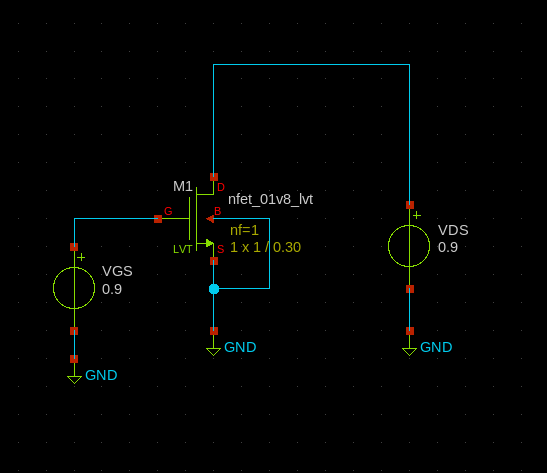
\includegraphics[width=\columnwidth]{schem.png}
	\caption{Schematic diagram}
	\label{schematic}
\end{figure}
At the minimum length, the intrinsic gain is lower than what is desired. $L=0.30\mu m$ is selected since it satisfies the specifications. $L=0.25\mu m$ also meets the specifications. However, for a greater swing, the larger length is selected. 
\begin{figure}[H]
	\centering 
	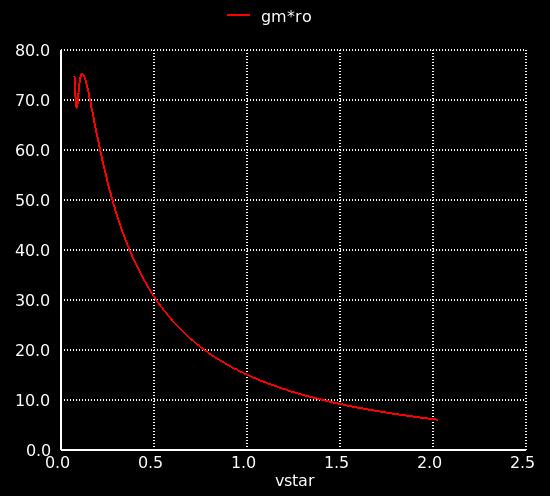
\includegraphics[scale=0.40]{gmro.png}
	\caption{Intrinsic gain}
	\label{gmro}
\end{figure}
The $V^*$ vs $I_D$ plot for a transistor with $W=1\mu m$, $L=0.30 \mu m$ is shown below. 
\begin{figure}[H]
	\centering 
	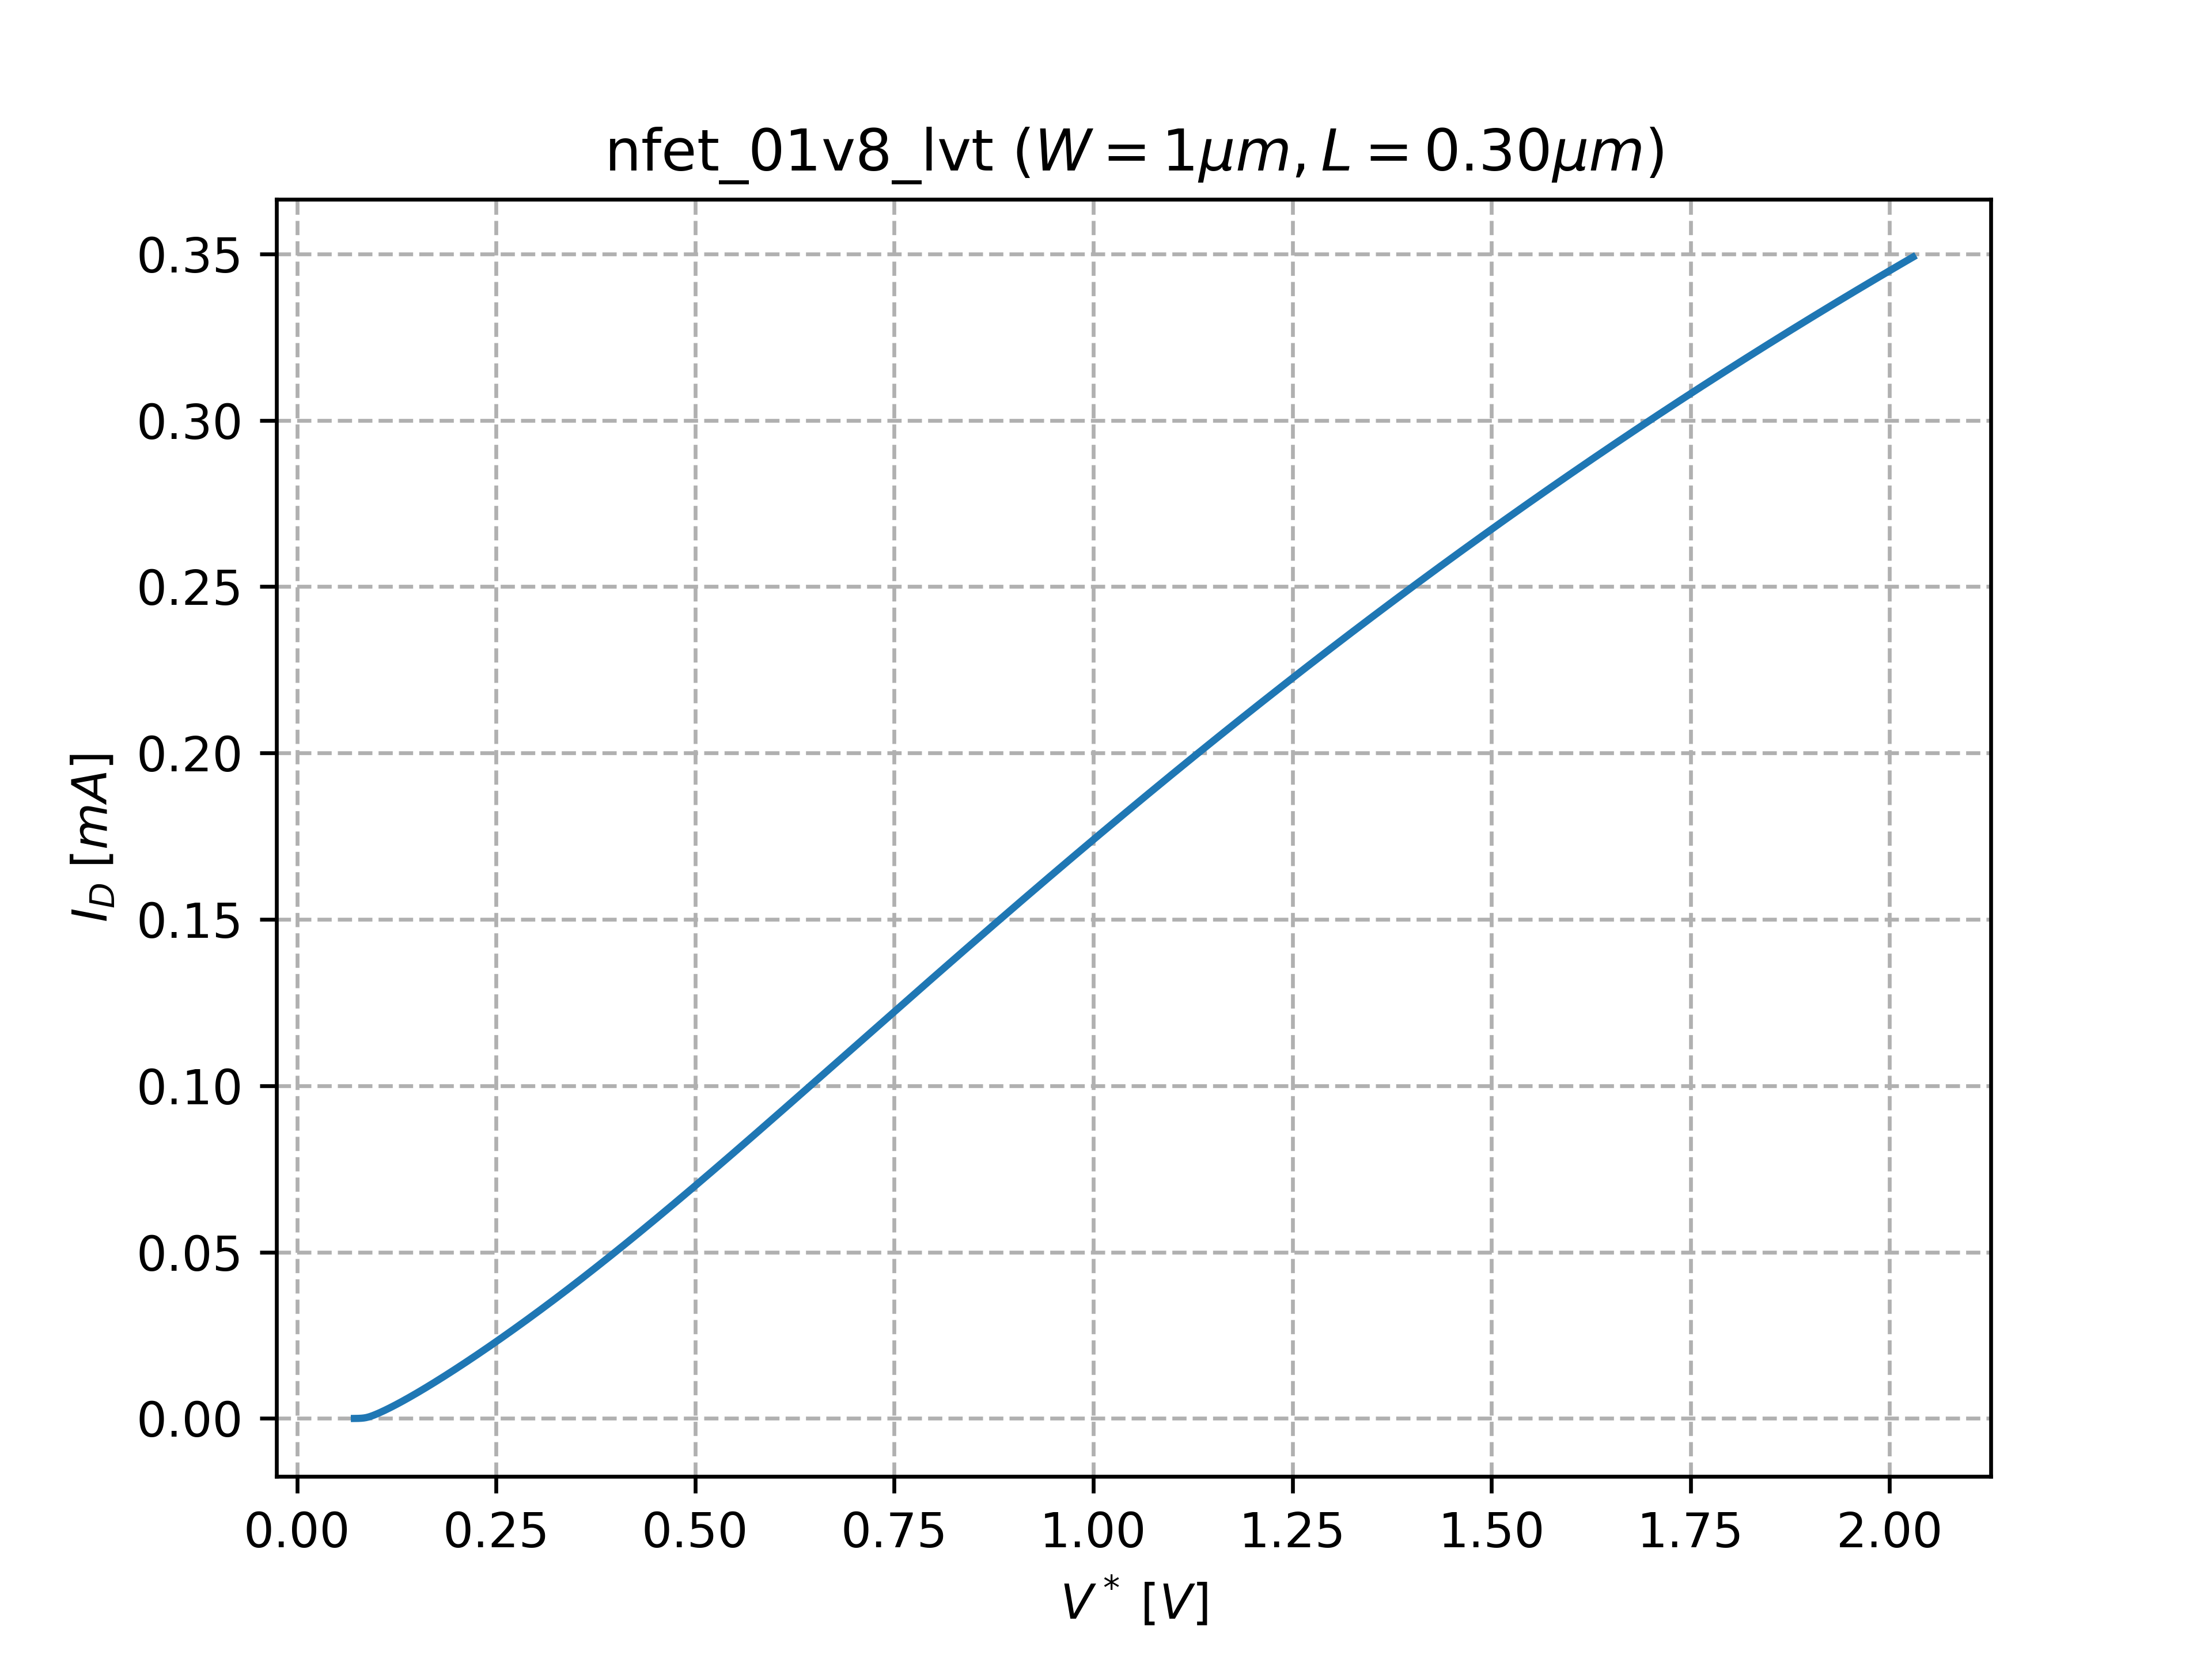
\includegraphics[scale=0.38]{vstar-id.png}
	\caption{$I_D$ vs $V^*$, $W=1\mu m$}
	\label{vstar-id}
\end{figure}
\subsection{Scaling the width}
A python script is used to calculate the scale factor $k_W$ that meets the required $I_D$. The width is scaled using $k_W$. Multiplying the width by $k_W$ scales $I_D$ by approximately the same factor. For this activity, $k_W=21$.
To check, a MEAS directive is used. The required current is $I_D=314\mu A$. Due to some estimates, $I_D=345\mu A$ is obtained.  
\begin{figure}[H]
	\centering 
	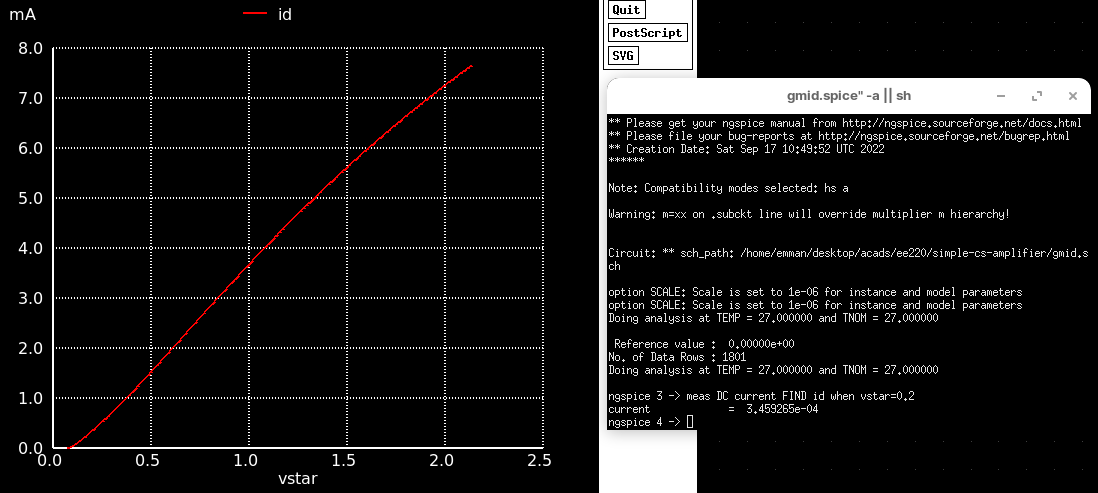
\includegraphics[width=\columnwidth]{vstar-scale-id.png}
	\caption{$I_D$ vs $V^*$, $W=21\mu m$}
	\label{vstar-scale-id}
\end{figure}
\subsection{Output and input swing}
\begin{figure}[H]
	\centering 
	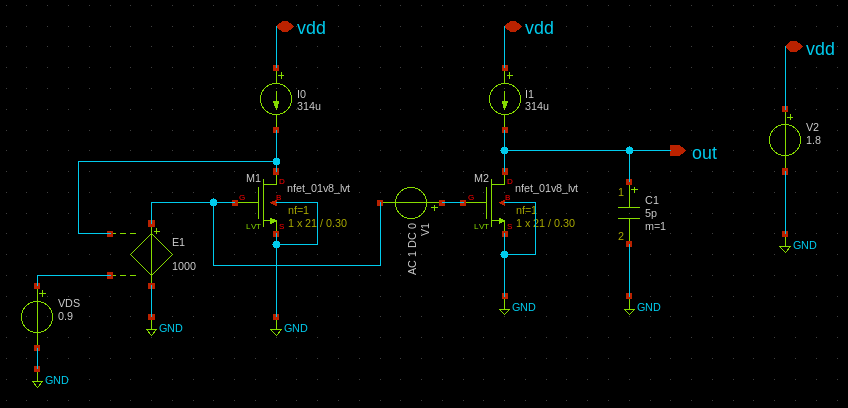
\includegraphics[width=\columnwidth]{schem_large.png}
	\caption{Schematic}
	\label{schem-large}
\end{figure}
To get the input and output swing, the schematic in Fig. \ref{schem-large} is used. Since 
$V_{GS}$ is a function of $V_{DS}$, $a_o$ vs $V_{DS}$ can be plotted to get the maximum output
swing and $a_o$ vs $V_{GS}$ to get the corresponding input swing. 

\vspace{8pt}
\subsubsection{Output Swing}
at $V_{DS}\approx 0.52$, $a_o \geq 40$. 
\begin{figure}[H]
	\centering 
	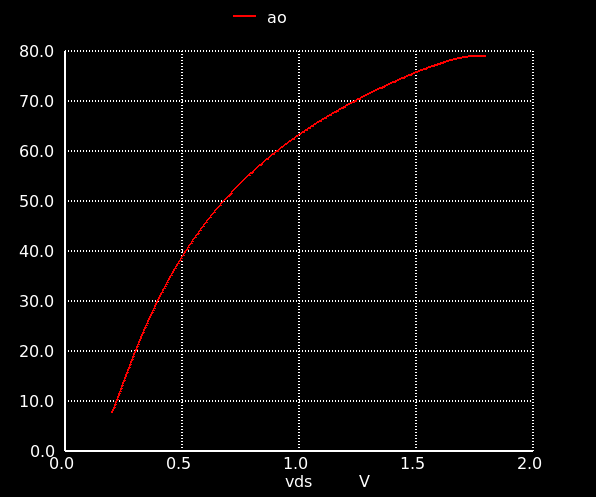
\includegraphics[scale=0.3]{ao-vds.png}
	\caption{$a_o$ vs $V_{DS}$}
	\label{swing-out}
\end{figure}
\subsubsection{Input Swing}
at $V_{GS}\approx 0.71$, $a_o \geq 40$. 
\begin{figure}[H]
	\centering 
	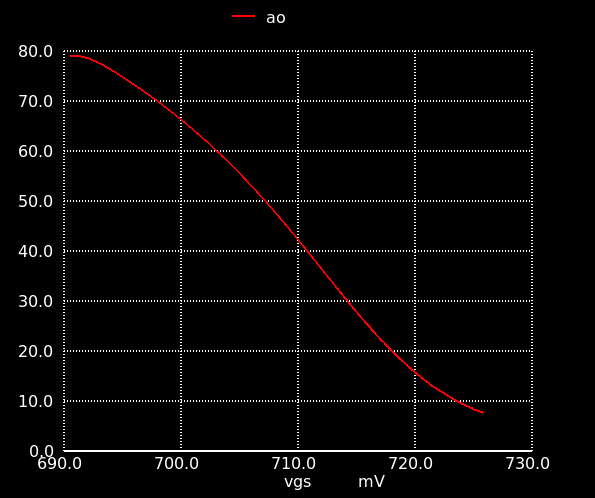
\includegraphics[scale=0.3]{ao-vgs.png}
	\caption{$a_o$ vs $V_{GS}$}
	\label{swing-in}
\end{figure}
Thus, the maximum symmetric output voltage is $0.52 \leq V_{DS} \leq 1.48$ for a total swing of $0.96V$. The corresponding input is $0.6946 \leq V_{GS} \leq 0.7106$ with a $16mV$ swing.
\vspace{8pt}
\subsubsection{Input vs output}
Shown in Fig. \ref{vinvout-1} is a sweep of $V1$ from $-8mV$ to $8mV$. 
\begin{figure}[H]
	\centering 
	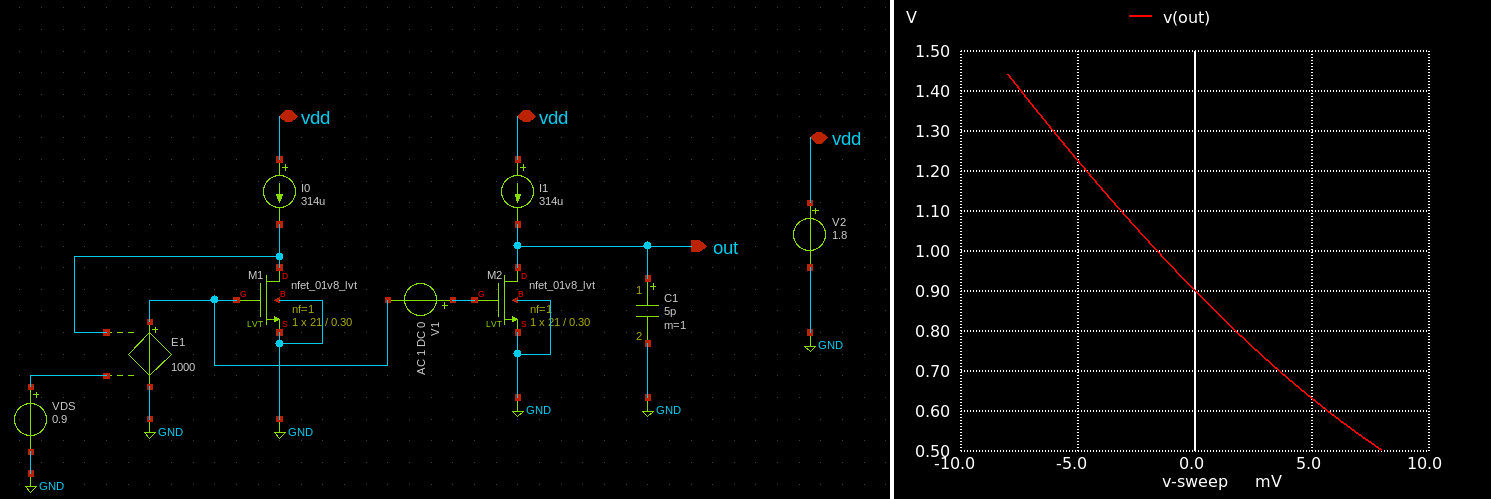
\includegraphics[width=\columnwidth]{v1-sweep-1.png}
	\caption{$a_o$ vs $V_{GS}$}
	\label{vinvout-1}
\end{figure}

\subsection{AC analysis}
Using Fig. \ref{schem-large}, an AC sweep from $1 Hz$ to $1GHz$ is performed. The resulting magnitude response plot is shown in Fig. \ref{vdb}. Using a MEAS directive, $f_u=104MHz$, which is close to the desired $f_u$. At low frequencies, the gain is $\approx 35dB$
which is $\approx 60\; V/V$
\begin{figure}[H]
	\centering 
	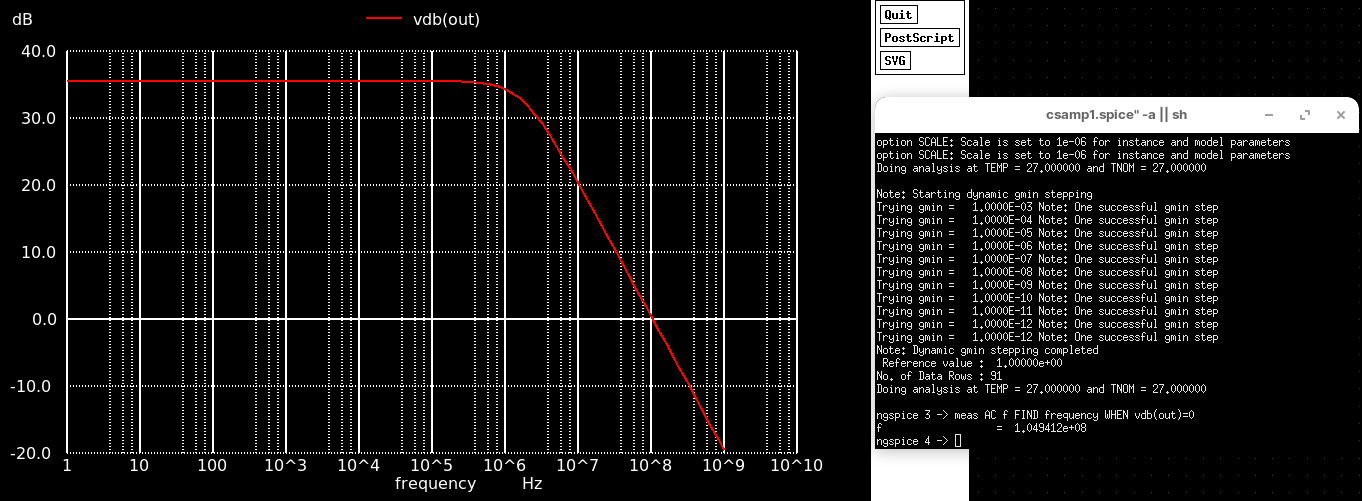
\includegraphics[width=\columnwidth]{vdb.png}
	\caption{Magnitude response}
	\label{vdb}
\end{figure}
\subsection{Discussions}
These are my expected results. Since some values are estimated, there are slight deviations with the desired specifications. 

\vspace{8pt}
\section{CS Amplifier with High $f_t$} 
To get a high $f_t$, a small $L$ and high power is required. Decreasing $L$ increases $f_t$ if $I_D$ is kept constant. However, since there are no constraints on area and how high $I_D$ could be, the limit would be related to the maximum $W$ that can be used on the PDK. 

\subsection{Selecting the width}
There is a trade-off between power and frequency. The higher the power that is used, the higher the frequency the circuit could get. Since $V_{DD}$ is fixed, the current consumption can be increased to bring more power to the circuit --- this is done by increasing the width. 


\vspace{8pt}
For this PDK, the largest width that can be used is $W=99.9\mu m$. This value is used to get the maximum $I_D$ that meets the specifications. All simulations for this part will use this value. 

\subsection{Choosing the length and $V^*$}
Ideally to get the highest $f_t$, the minimum length should be selected. However, the minimum length does not have sufficient intrinsic gain. Since the load is an ideal current source, the gain is only limited by the lower bound $\approx 700mV$. $V_{DS}=0.7V$ is used for this characterization part. 

\vspace{8pt}
\subsubsection{$a_o$ vs $V^*$} 
For $0.20\mu m \leq L \leq 0.25\mu m$, the $a_o$ vs $V^*$ plot is shown below. 
\begin{figure}[H]
	\centering 
	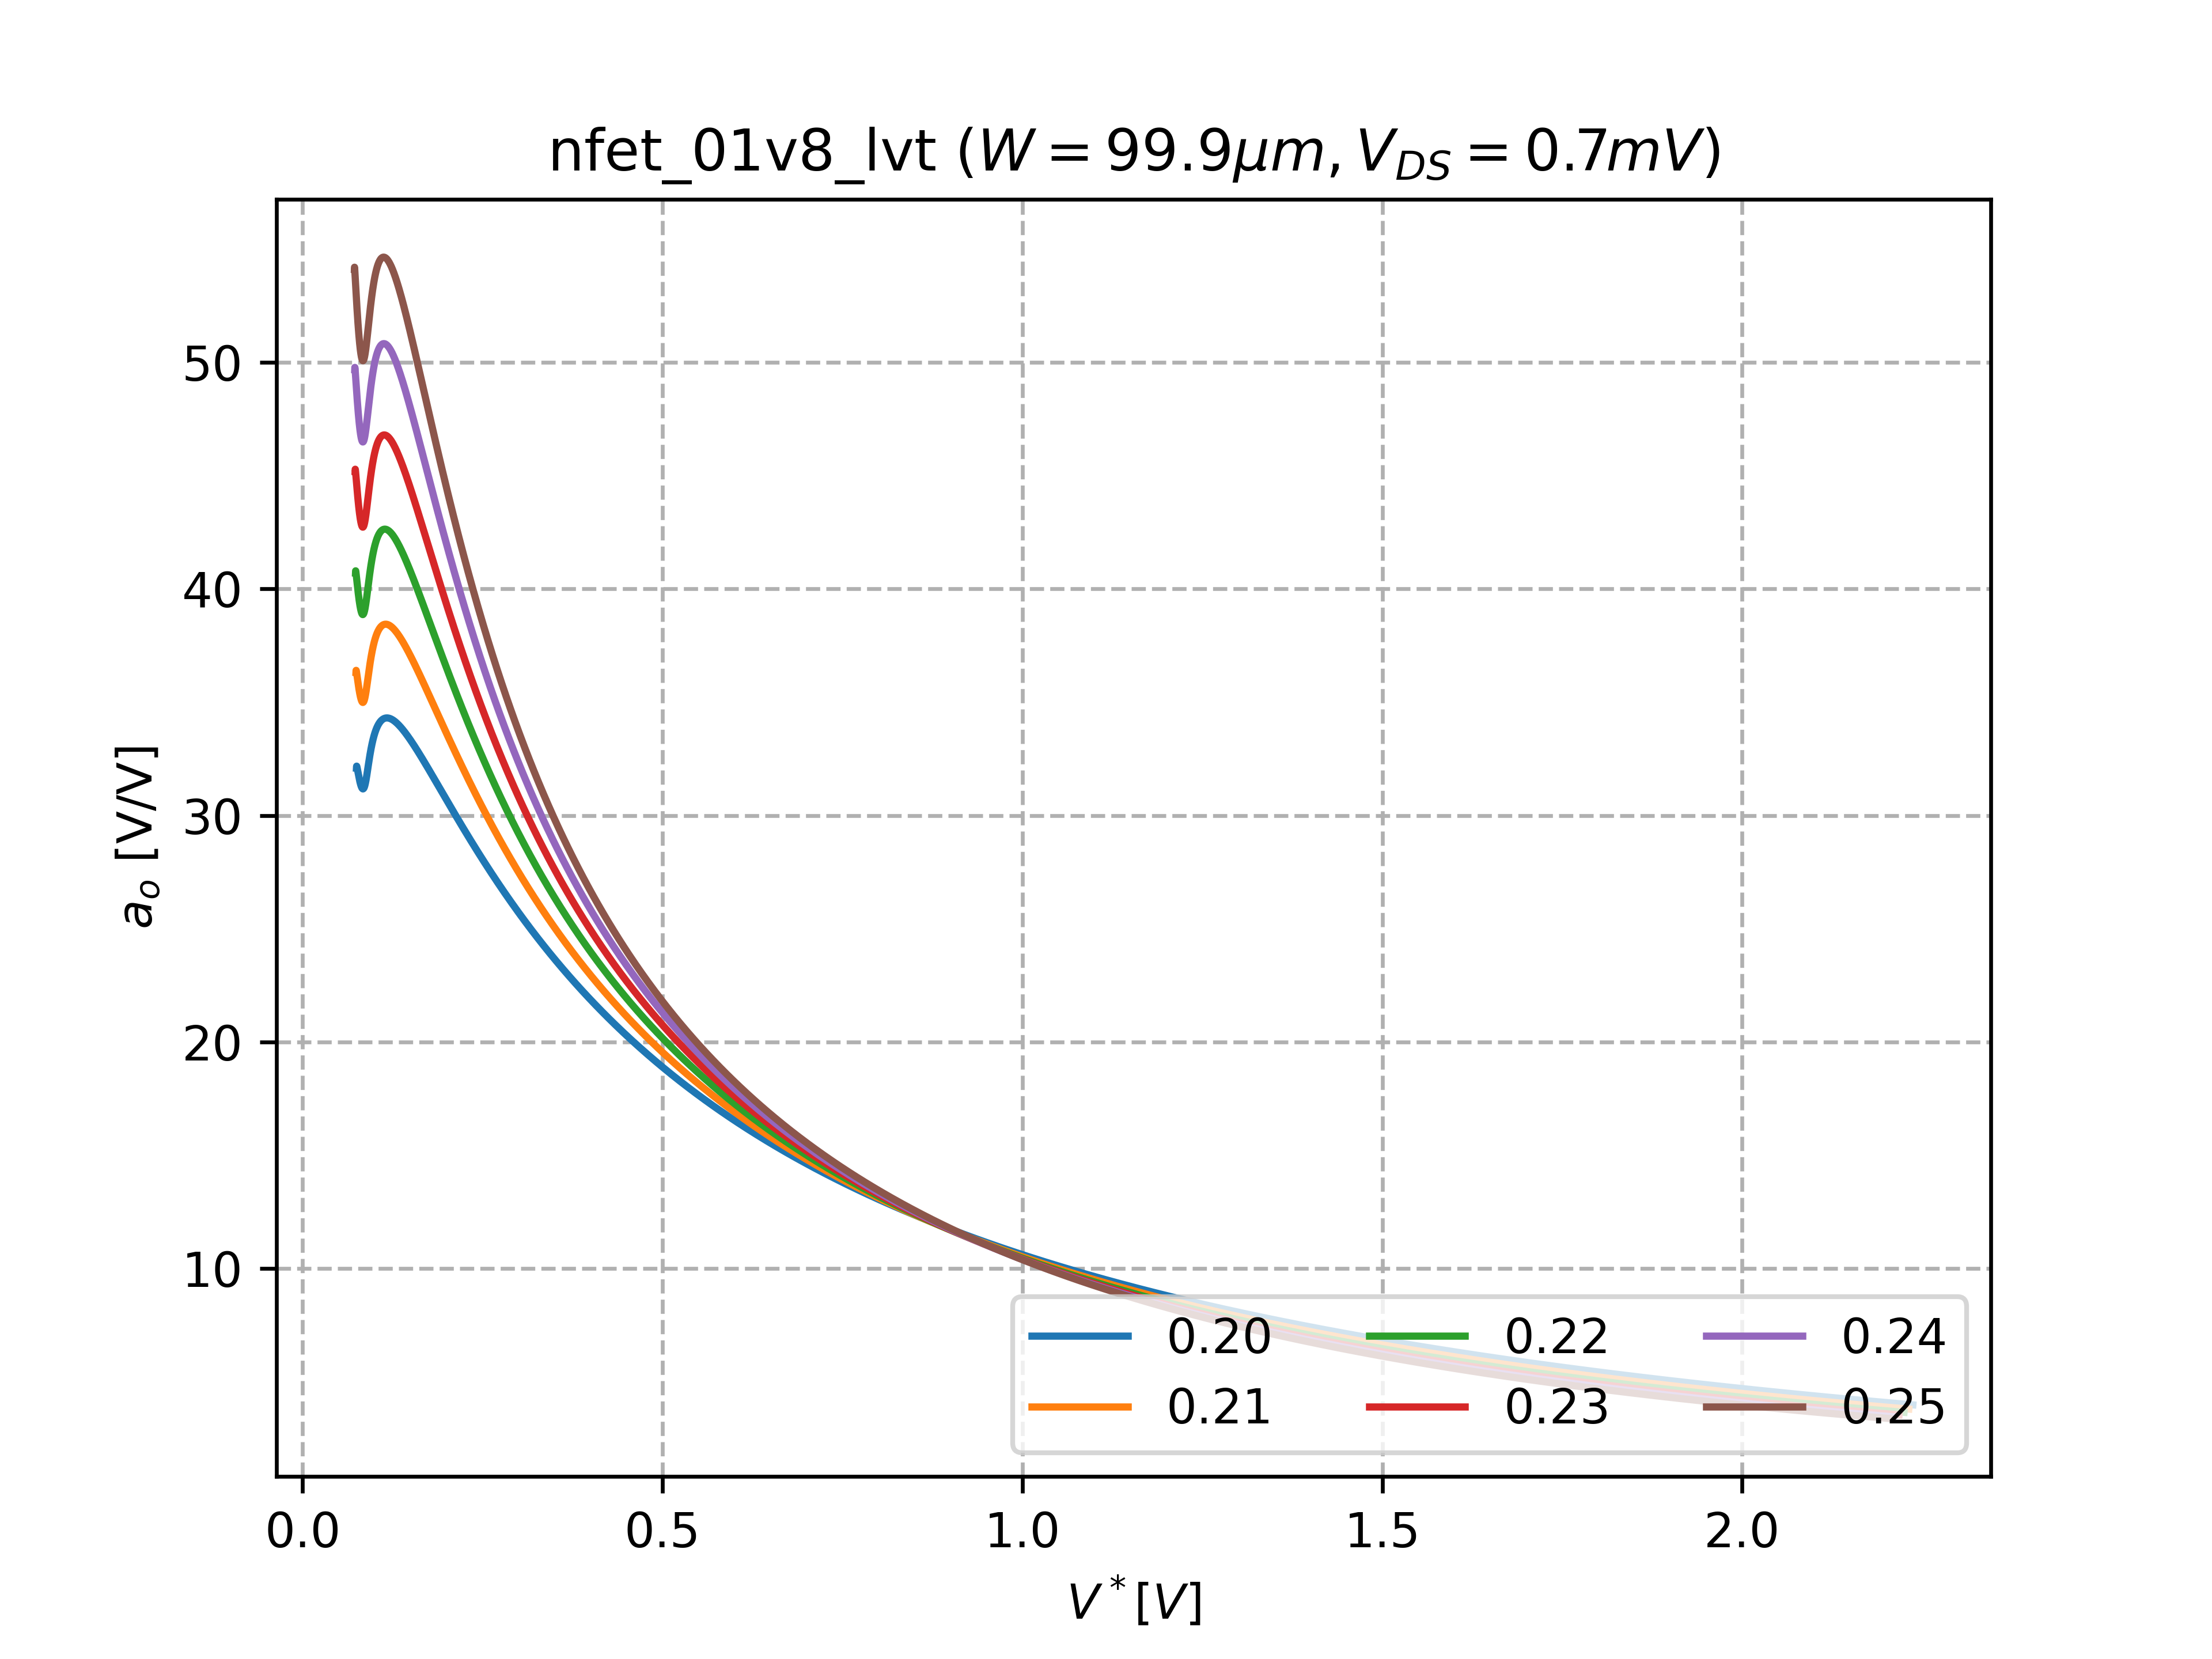
\includegraphics[width=\columnwidth]{vstar-ao-maxft.png}
	\caption{Intrinsic gain}
	\label{vstar-ao-2}	
\end{figure}
Since the desired gain is $a_o > 40$, only lengths $\geq 0.22\mu m$ can be used. 

\vspace{8pt}
\subsubsection{$f_t$ vs $V^*$} 
To trim down the possible options, an $f_t$ vs $V^*$ plot is used. 
 
\begin{figure}[H]
	\centering 
	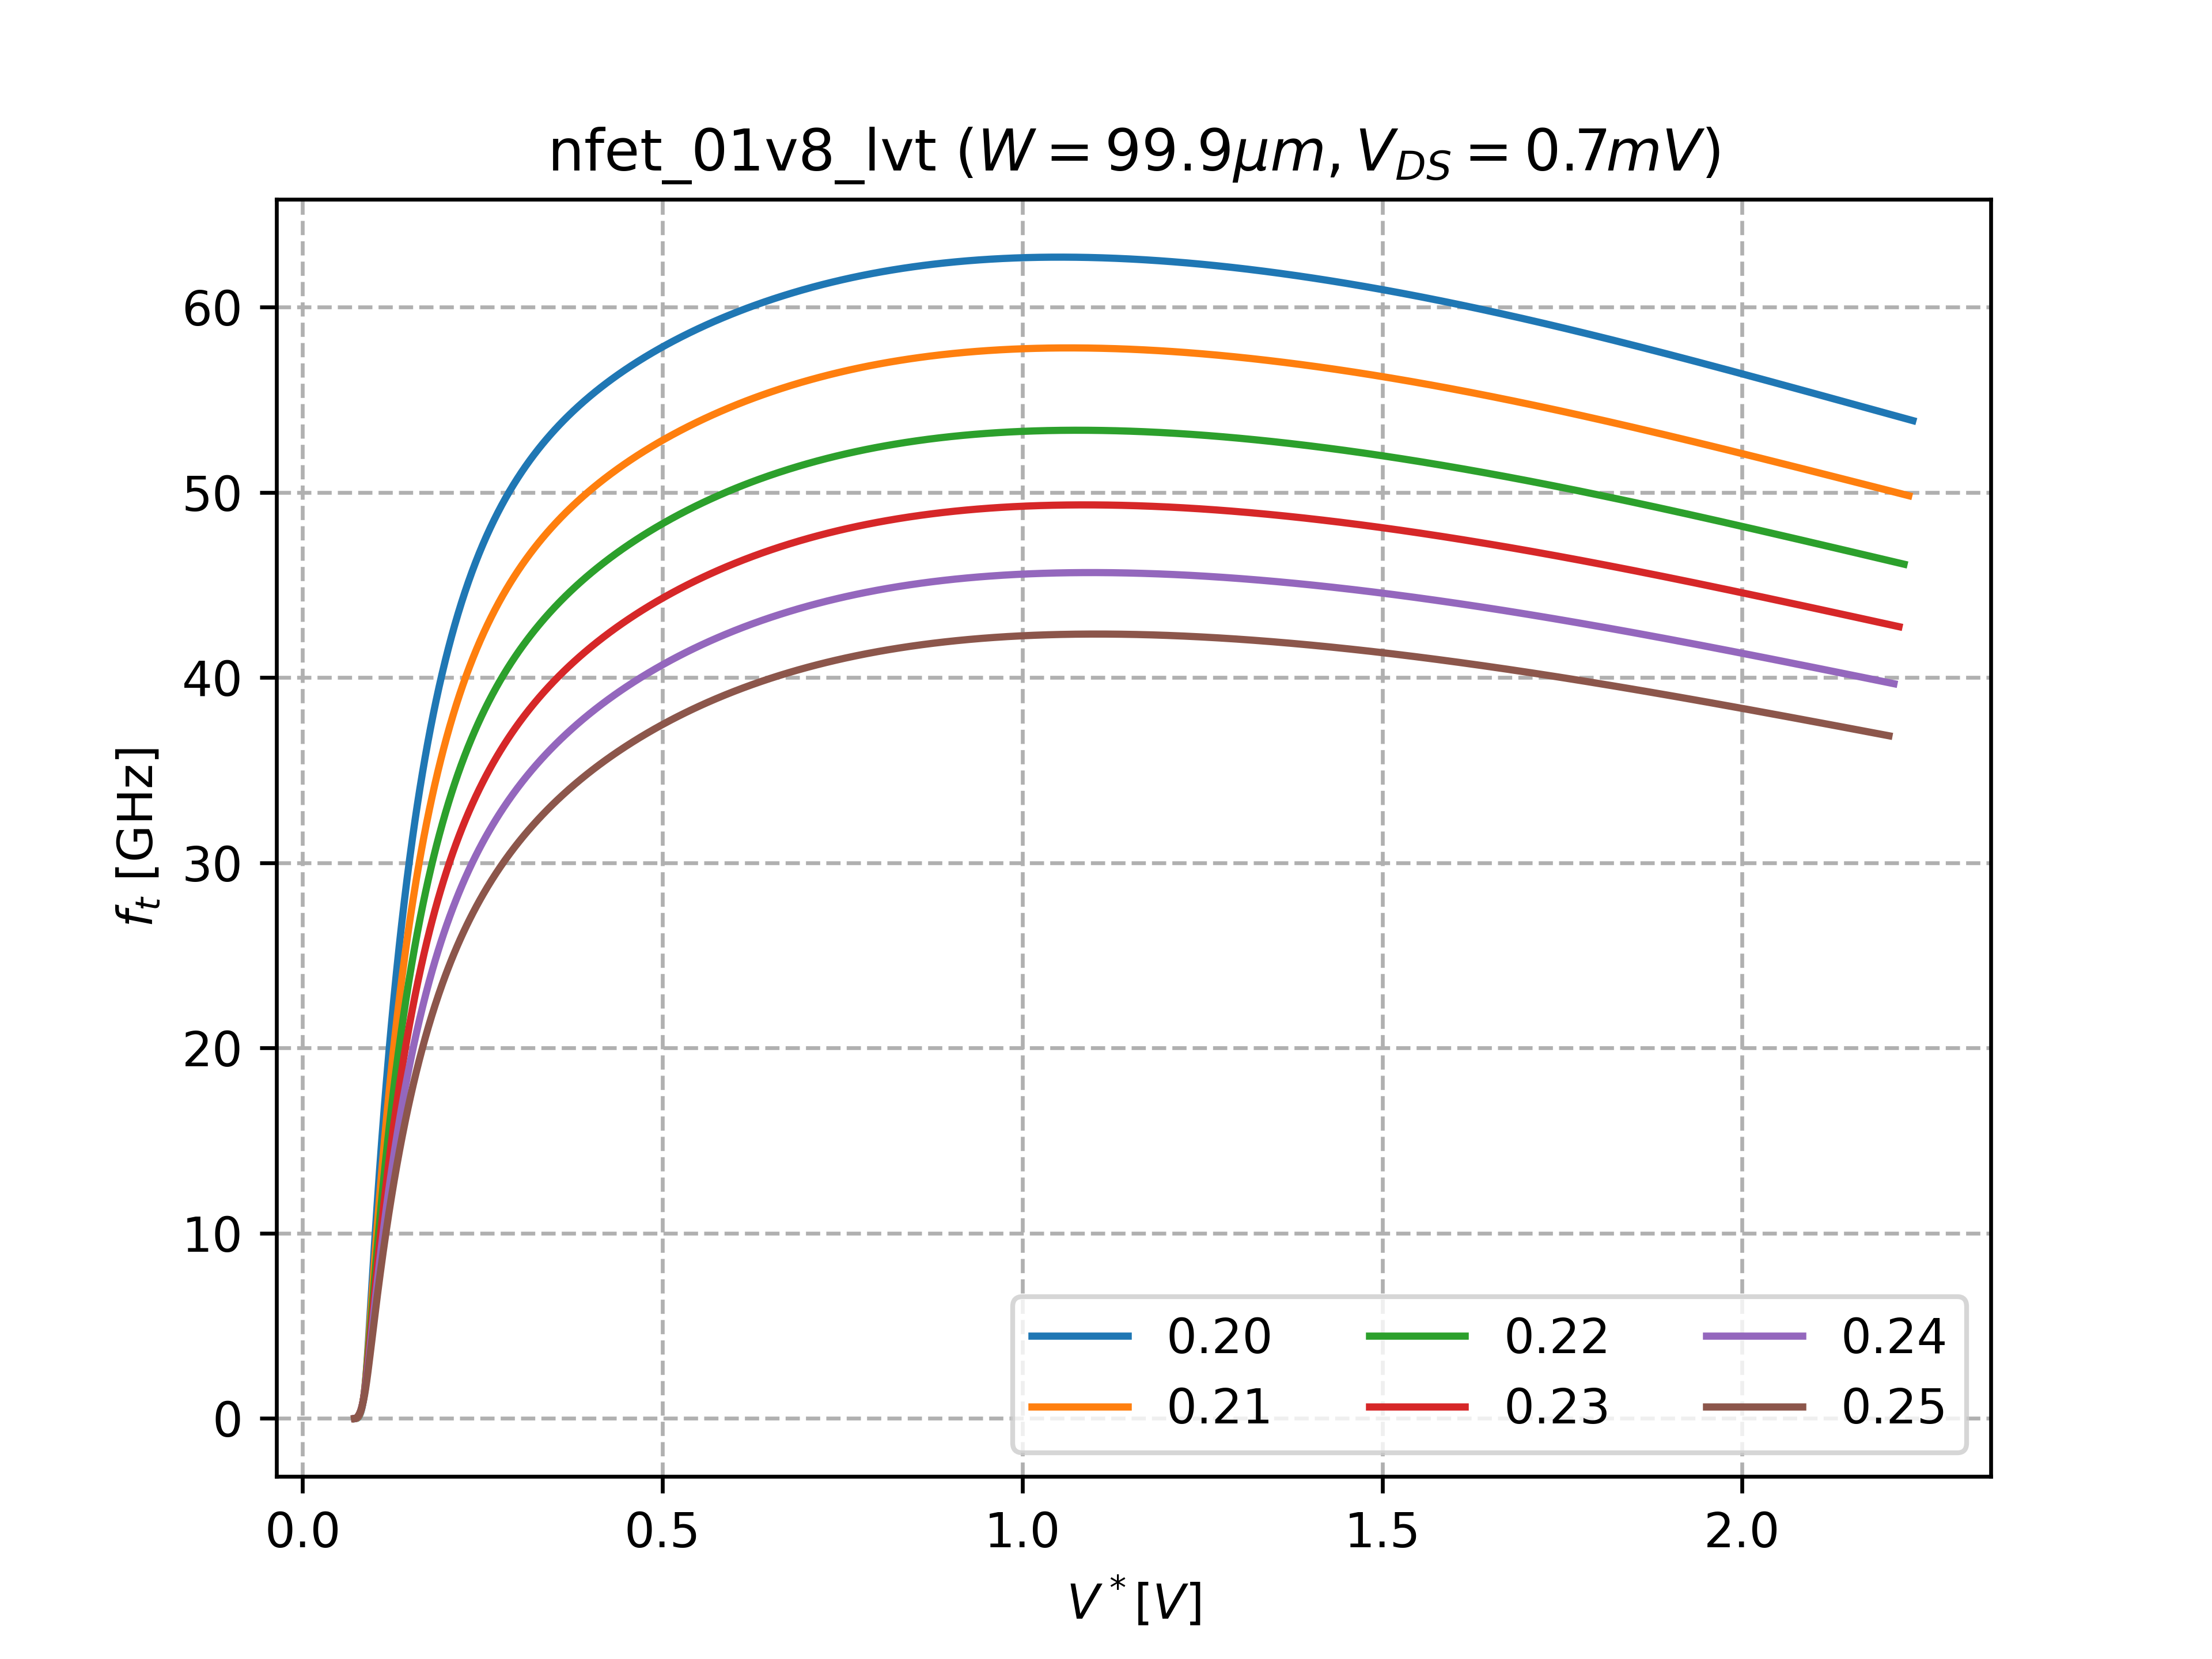
\includegraphics[width=\columnwidth]{vstar-ft-maxft.png}
	\caption{Transition frequency}
	\label{vstar-ft-2}	
\end{figure}
Considering the two plots, $V^*=0.19V$ and $L=0.23\mu m$ are chosen since they lead to the highest $f_t$. The gain and swing at these values are also within the required specifications. The obtained $f_t$ is $28GHz$.
\subsection{Obtaining $g_m$ and $f_u$}
\begin{figure}[H]
	\centering 
	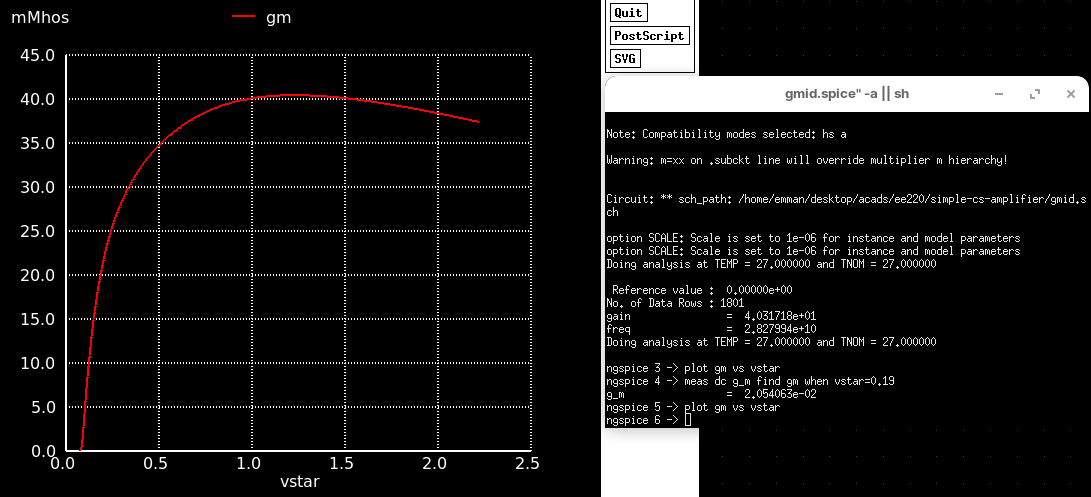
\includegraphics[width=\columnwidth]{gm-vstar.png}
	\caption{$g_m$ vs $V^*$}
	\label{gm-vstar}	
\end{figure}
From Fig. \ref{gm-vstar}, $g_m=20.54mS$ at $V^*=0.19V$. The target unity-gain frequency is:
\begin{equation*}
	f_u = \frac{g_m}{2\pi C_L} = 653.81MHz
\end{equation*}
with $I_D=1.95mA$. 
\subsection{AC analysis}
\begin{figure}[H]
	\centering 
	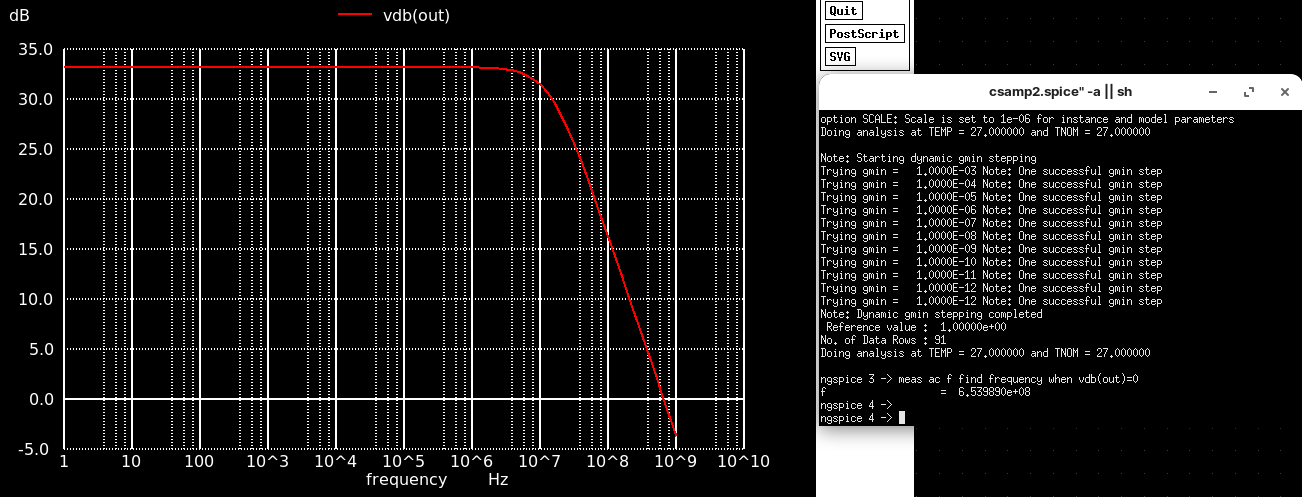
\includegraphics[width=\columnwidth]{fumax.png}
	\caption{Unity-gain frequency}
	\label{fu-vstar}	
\end{figure}
Looking at Fig. \ref{fu-vstar}, $f_u \approx 654MHz$. The desired $f_u$ is met. At low frequencies, the gain is $33.19\; dB$ which corresponds to $45.66\; V/V$.
\subsection{Output and input swing}
\subsubsection{Output Swing}
From the plot below, it is seen that $a_o=40.32$ at $V_{DS}=0.7$. At $V_{DS}=1.1$, $a_o\approx 50$.
\begin{figure}[H]
	\centering 
	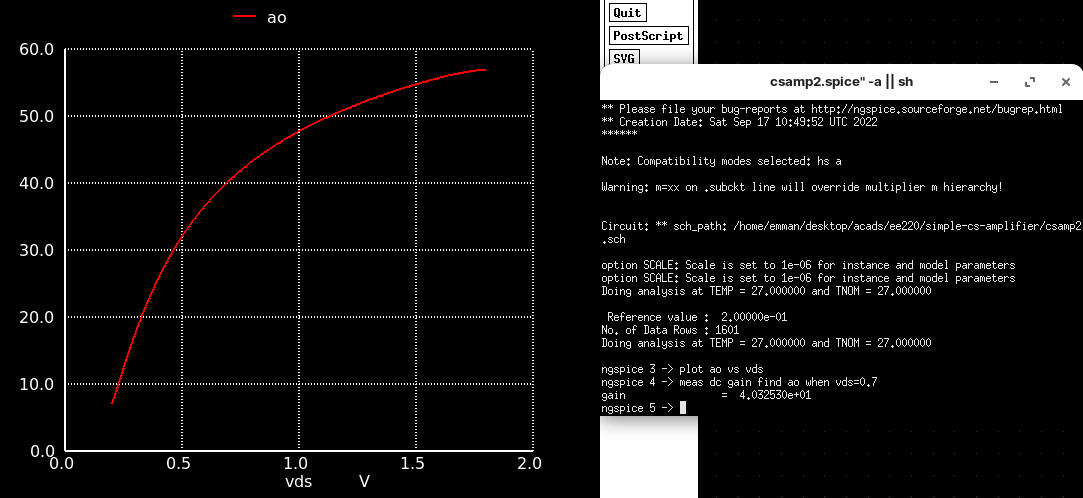
\includegraphics[width=\columnwidth]{gain-fumax-vds.png}
	\caption{$a_o$ vs $V_{DS}$}
	\label{ao-fumax-vds}	
\end{figure}
\subsubsection{Input Swing}
Sweeping $V_{DS}$ from $700mV$ to $1.1V$, the following $a_o$ vs $V_{GS}$ plot is obtained. 
The input $V_{GS}$ that produces $700mV \leq V_{DS} \leq 1.1V$ ranges from $719mV$ to $727mV$. 
The maximum swing is $8mV$. 
\begin{figure}[H]
	\centering 
	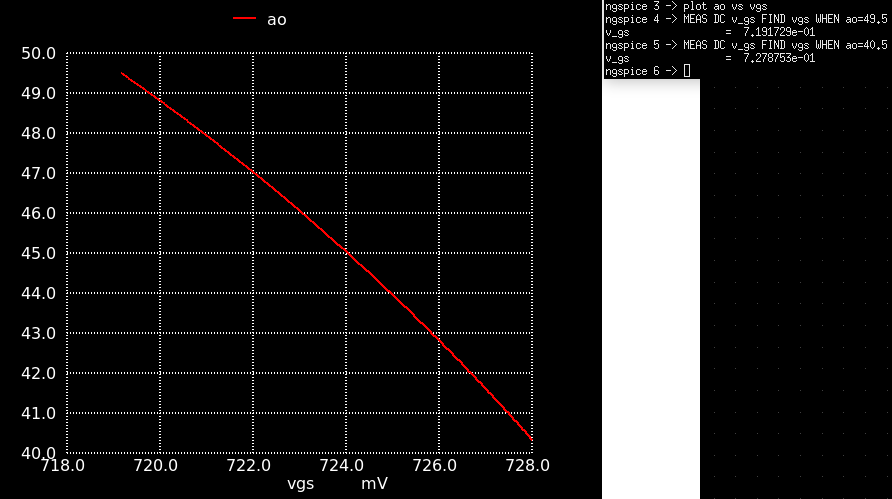
\includegraphics[width=\columnwidth]{gain-fumax-vgs.png}
	\caption{$a_o$ vs $V_{GS}$}
	\label{ao-fumax-vgs}	
\end{figure}
\subsubsection{Input vs output}
$v_{in}$ is swept from $-4mV$ to $4mV$ to get the corresponding $v_{out}$. 
\begin{figure}[H]
	\centering 
	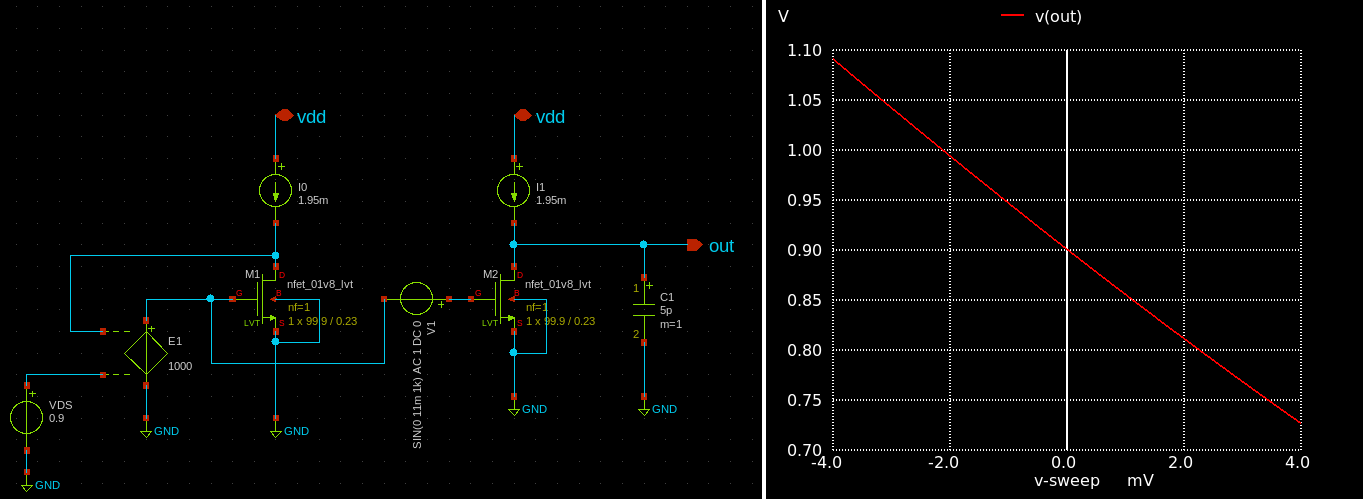
\includegraphics[width=\columnwidth]{vinvout.png}
	\caption{$v_{in}$ vs $v_{out}$}
	\label{vinvout-2}	
\end{figure}

\subsection{Discussions}
First, the choice of $V^*$ depends on both gain and desired $f_t$. If we increase $V^*$, we 
can get a higher $f_t$ but the gain will decrease. To maximize $f_t$, the maximum $V^*$ that 
satisfies both gain and swing should be chosen. This amplifier is designed to have an approximate output swing of $\pm 200mV$ with a DC level of $0.9V$ because of $f_t$ constraints. 

\vspace{8pt}
The first design has $I_D = 314\mu A$. For this design, $I_D=1.95mA$. The $I_D$ is more than 6 times higher. RF applications would benefit from a high $f_u$ but this might not be usable at all because of very high current consumption. 







\end{document} 
